%!TEX root = ../main.tex

\section{Hardware Description}
The project includes many parts that must be combined to make the kart actually drive. 
A short description of each part is made to provide an overview of the system.

\subsection{Go-Kart Frame}
The Go-Kart itself consists of a pre assembled aluminium frame with wheels, steering column, break pedal and seat all pre-attached to the frame. 
Behind the seat a plate is attached to fit all of the power electronics and drive systems that are designed throughout this project.
To the right of the driver a mount is positioned for the motor.
The mount is protected by a metal cover. 
In order to properly transfer energy to the rear wheels, a gearing is placed between the motor and the rear axle.
A conventional disc brake comes pre-installed on the kart with the break pedal connected using hydraulic fluid.
The speeder pedal is also installed, but nothing is attached to it, so it has no function initially.

\todo[inline]{It has no mechanical effetct? but will work with the sevcon - Mikkel}
\todo[inline]{Thomas: Surely this is no longer the case?}
\begin{figure}[!h]
	\centering
	\begin{subfigure}[t]{.35\linewidth}
		\includegraphics[width=\textwidth]{graphics/Gokart_Frame}
		\caption{The frame of the go-kart used in this project.}
		\label{fig:Kart_picture1}
	\end{subfigure}
	\hspace{2cm}
	\begin{subfigure}[t]{.35\linewidth}
		\includegraphics[width=\textwidth]{graphics/me1117_1}
		\caption{The Me1117 PMAC motor mounted on the go-kart.}
		\label{fig:The Me1117 PMAC}
	\end{subfigure}		
	\caption{Go-kart and PMAC motor.}
	\label{fig:Motor_picture1}
\end{figure}
\todo{better pic of motor}

\subsection{Battery Supply}
\todo[inline]{Thomas: We need to discuss whether units should be in math mode or in text!}
The batteries provided for this project are called: "SB12V20P-FC Super B
Lightweight Lithium Ion starter battery". \todo{cite datasheet}
Four of these batteries will be put in series, yielding a combined nominal voltage of 52.8V and a discharge current of 560A. The discharge current can go up to as much as 1200A for a second.
The batteries are relatively small at $\approx 238x120x82mm$ and $3.2kg$ of weight each.
The batteries will be providing all the required power for the go-kart, including the motor and all control and drive circuits.

\todo[inline]{We will put in extra batteries for the fans though - Mikkel}

\subsection{PMAC Motor}
The PMAC motor provided is a three phase motor capable of 

\todo[inline]{Thoms: very little it seems...}

\subsection{Torque Pedal}
The torque pedal or "speeder" is provided as well. 
It consists of a levered variable resistor with the equivalent diagram seen in figure \ref{fig:Torque_pedal_diagram}.
\todo{Thomas: you should fix your references grrr..}

The torque pedal will be used to control the speed by increasing or lowering the resistance, resulting in a change in voltage on the return wire. 
By measurement, it is found to have a variable resistance of 0k to 7.5k.
It is also found to be inaccurate in the decimals while holding a position, meaning some kind of filter might be necessary.

\todo[inline]{Inaccurate in the decimals? How is this measured? Maybe your hand was shaking? But yeah, we might need filtering - Mikkel}


\begin{figure}[!h]
	\centering
	\begin{subfigure}[t]{.35\linewidth}
			\includegraphics[width=\textwidth]{graphics/torque_pedal_diagram}
			\caption{Diagram of the torque pedal}
			\label{fig:Torque_pedal_diagram}
	\end{subfigure}
	\hspace{2cm}
	\begin{subfigure}[t]{.35\linewidth}
		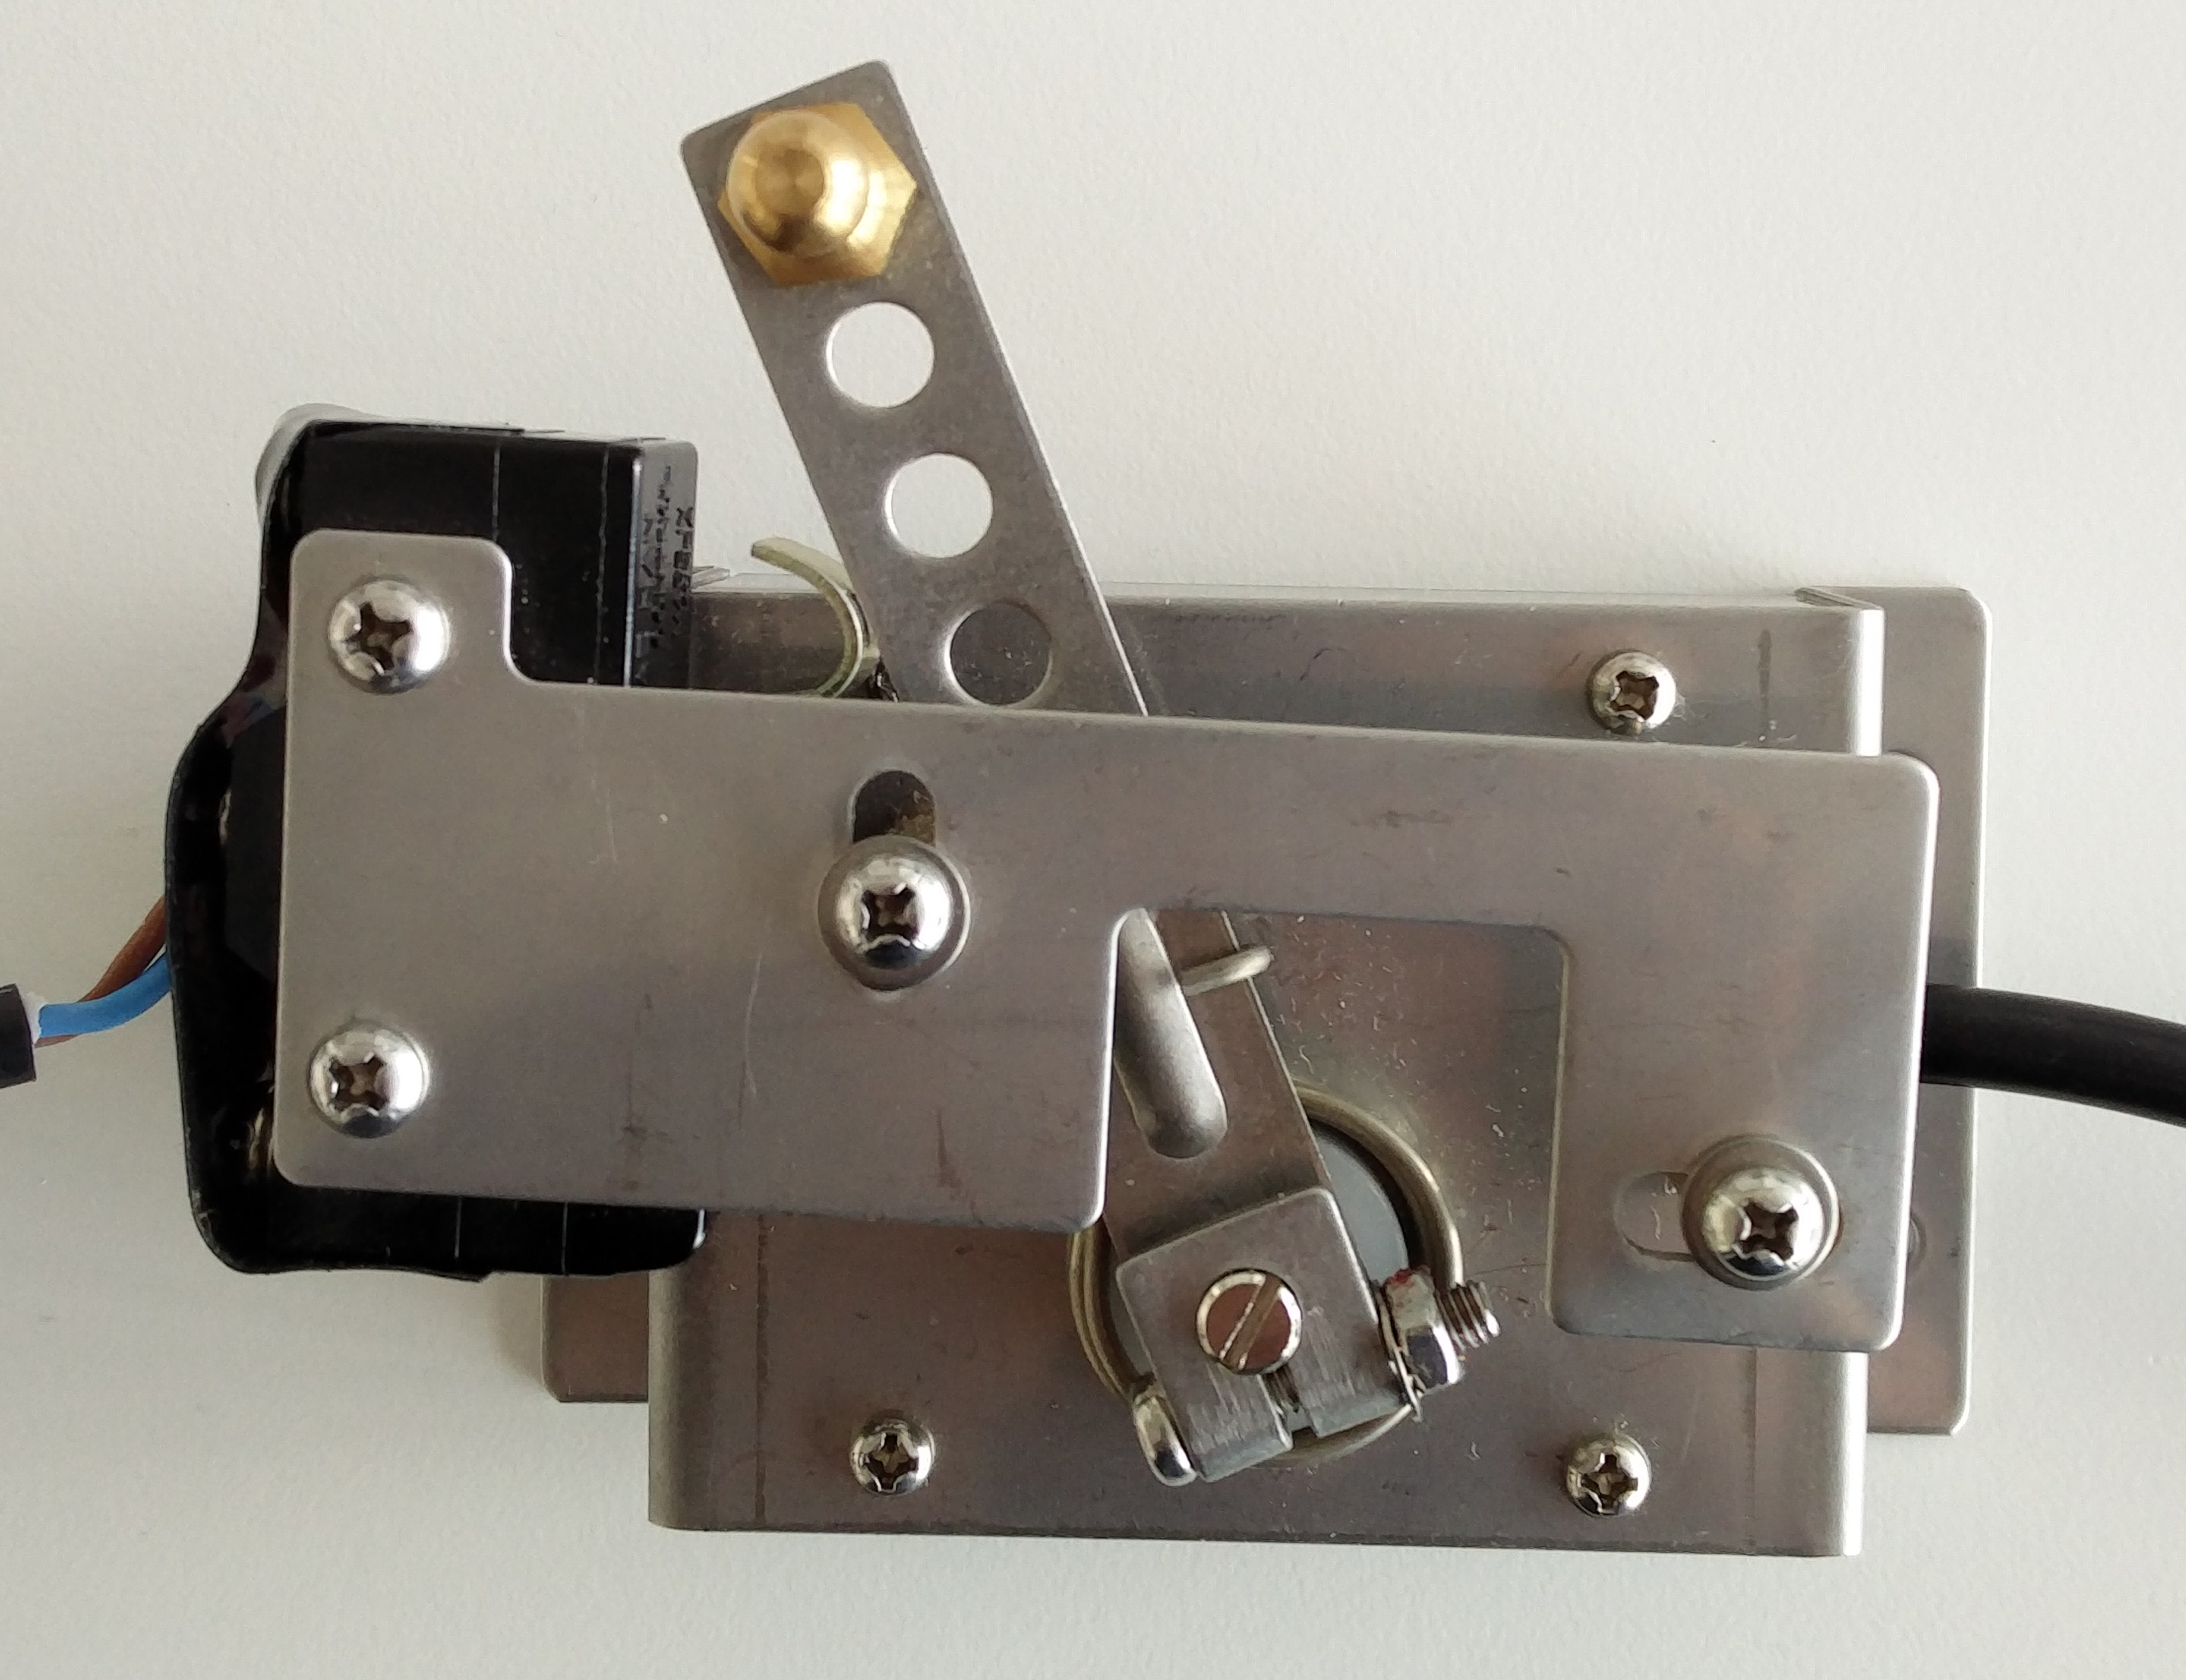
\includegraphics[width=\textwidth]{graphics/torque_pedal_picture}
		\caption{Picture of the actual torque pedal}
		\label{fig:Torque_pedal_picture}
	\end{subfigure}
	\caption{Diagram and picture of the torque pedal}
	\label{fig:Torque_pedal_diagram}
\end{figure}

\subsection{Switches and Wiring}
The wiring of the kart frame is not pre-assembled, but has been provided by the supervisors of the project, as this is standardized across multiple projects. 
A diagram of the wiring can be seen on figure \ref{fig:Kart_wiring_diagram}.\newline

The diagram shows the Sevcon Gen4 controller as the centrepiece surrounded by the other active parts. 
The motor to the right. 
The torque pedal, battery, undervoltage protection and multiple switches to the left. 
The switches include a key switch to turn the system on, an emergency switch, and a drive enable switch with three positions to change between driving forwards, reversing or disabling drive at the neutral position.

\begin{figure}[!h]
	\centering
	\includegraphics[width=.95\linewidth]{graphics/Electrical_wiring_diagram_ver3}
	\caption{Go-Kart wiring diagram}
	\label{fig:Kart_wiring_diagram}
\end{figure}

\clearpage